\documentclass[runningheads]{llncs}
%
% \documentclass[sigplan,10pt,anonymous,review]{acmart}\settopmatter{printfolios=true,printccs=false,printacmref=false}

\usepackage[T1]{fontenc}
\usepackage[utf8]{inputenc}
\usepackage{microtype} % Better typesetting for PDFs -- is enabling this ok?
\usepackage{balance}

\usepackage{amsmath}
\usepackage{amssymb}
% \usepackage{amsthm}

%\usepackage{eufrak} %The eufrak package is redundant if the amsfonts package is used
\usepackage{mathpartir}
\DeclareMathAlphabet{\mathpzc}{OT1}{pzc}{m}{it}
\usepackage[boxed]{algorithm}
\usepackage{enumerate}
\usepackage{cprotect}

\usepackage{listings}
\usepackage{lstautogobble}
\usepackage{graphicx}
\usepackage{tabularx}
\usepackage{booktabs}
\usepackage{ragged2e}  % for '\RaggedRight' macro (allows hyphenation)
\usepackage{color}
\usepackage[noend]{algpseudocode}
\usepackage{caption}
\usepackage[font=scriptsize]{subcaption}
\usepackage{hyperref}
\usepackage{float}
\usepackage{wrapfig}

\usepackage{multirow}
\usepackage{siunitx}


\usepackage{tikz}
\usetikzlibrary{positioning,fit,shadows,decorations, arrows, shapes, decorations.markings,decorations.pathmorphing,calc}

\usepackage{pgfplots}


\tikzset{
  -|-/.style={
    to path={
      (\tikztostart) -| ($(\tikztostart)!#1!(\tikztotarget)$) |- (\tikztotarget)
      \tikztonodes
    }
  },
  -|-/.default=0.5,
  |-|/.style={
    to path={
      (\tikztostart) |- ($(\tikztostart)!#1!(\tikztotarget)$) -| (\tikztotarget)
      \tikztonodes
    }
  },
  |-|/.default=0.5,
}

\clubpenalty = 10000
\widowpenalty = 10000
\displaywidowpenalty = 10000

% Not really meant for highlighting isabelle source, but for easily writing latex that looks like
% isabelle
% 
% keyword level 1 - isabelle outer syntax 
% keyword level 2 - isabelle inner syntax programming constructs (if, let, etc)
% keyword level 3 - standard constants (length, mod, etc)
% keyword level 4 - isabelle proof methods


% \newcommand{\lsem}{\ensuremath{\mathopen{[\![}}}
% \newcommand{\rsem}{\ensuremath{\mathclose{]\!]}}}

\lstdefinelanguage{isabelle}{
  morekeywords={theorem,theorems,corollary,lemma,lemmas,locale,begin,end,fixes,assumes,shows,and,class,
    constrains , definition, where, apply, done,unfolding, primrec, fun, using, by, for, uses, file,
    schematic_lemma, concrete_definition, prepare_code_thms, export_code, datatype, type_synonym, typedef, value,
    proof, next, qed, show, have, hence, thus, interpretation, fix, context, sepref_definition,is,export_llvm
 } ,
  morekeywords=[2]{rec, return, bind, foreach, if, then, else, do, let, in, res, spec, fail, assert, while, case, of, 
    check},
%  morekeywords=[3]{length,mod,insert},
%   morekeywords=[4]{simp,auto,intro,elim,rprems,refine_mono,refine_rcg},
  sensitive=True,
  morecomment=[s]{(\*}{\*)},
}


\DeclareTextCommand{\shortunderscore}{T1}{{$\lambda$}}1
  {\\\%}{{$\lambda$}}1
  {\\\$}{{$\mathbin{\,\$\,}$}}1
  {->}{{$\rightarrow$}}1
  {<-}{{$\leftarrow$}}1
  {<.}{{$\langle$}}1
  {.>}{{$\rangle$}}1
  {<=}{{$\le$}}1
  {>=}{{$\ge$}}1
  {<->}{{$\leftrightarrow$}}1
  {-->}{{$\longrightarrow$}}2
  {<-->}{{$\longleftrightarrow$}}1
  {=>}{{$\Rightarrow$}}1
  {==}{{$\equiv$}}2
  {==>}{{$\implies$}}2
  {<=>}{{$\Leftrightarrow$}}1
  {~=}{{$\ne$}}1
  {|}{{$\mid$}}1
  {-`}{{$\rightharpoonup$}}1
  {|`}{{$\restriction$}}1
  {!!}{{$\bigwedge$}}1
  {(}{{$($}}1
  {)}{{$)$}}1
  {\{}{{$\{$}}1
  {\}}{{$\}$}}1
  {[}{{$[$}}1
  {]}{{$]$}}1
  {[|}{{$\llbracket$}}1
  {|]}{{$\rrbracket$}}1
  {\\<lbrakk>}{{$\lsem$}}1
  {\\<rbrakk>}{{$\rsem$}}1
  {|-}{{$\vdash$}}1
  {|=}{{$\models$}}1
  {|->}{{$\mapsto$}}1
  {|_|}{{$\bigsqcup$}}1
  {...}{{$\dots$}}1
  {\\x}{{$\times$}}1
  {_0}{{${}_0$}}1
  {_1}{{${}_1$}}1
  {_2}{{${}_2$}}1
  {_3}{{${}_3$}}1
  {_4}{{${}_4$}}1
  {_5}{{${}_5$}}1
  {_6}{{${}_6$}}1
  {_7}{{${}_7$}}1
  {_8}{{${}_8$}}1
  {_9}{{${}_9$}}1
  {_L}{{${}_L$}}1
  {\\_n}{{${}_n$}}1
  {\\_i}{{${}_i$}}1
  {\\_j}{{${}_j$}}1
  {\\_x}{{${}_x$}}1
  {\\_y}{{${}_y$}}1
  {\\impl}{{${}_\dagger$}}1
  {^*}{{$^*$}}1
  {^k}{{$^k$}}1
  {^d}{{$^d$}}1
  {\\<^sup>*}{{$^*$}}1
  {\\<^sub>*}{{$_*$}}1
  {\\<^sub>A}{{$_A$}}1
  {\\<^sub>r}{{$_r$}}1
  {\\<^sub>a}{{$_a$}}1
  {:_i}{{$:_i$}}1
  {\\<A>}{{$\mathcal{A}$}}1
  {\\<O>}{{\sf o}}1
  {\\<Phi>}{{$\Phi$}}1
  {\\<Psi>}{{$\Psi$}}1
  {\\<sigma>}{{$\sigma$}}1
  {\\<cdot>}{{$\cdot$}}1
  {\\<in>}{{$\in$}}1
  {\\<le>}{{$\le$}}1
  {\\<noteq>}{{$\ne$}}1
  {\\<lambda>}{{$\lambda$}}1
  {\\<longrightarrow>}{{$\longrightarrow$}}1
  {\\<longleftrightarrow>}{{$\longleftrightarrow$}}1
  {\\<Rightarrow>}{{$\Rightarrow$}}1
  {\\<Longrightarrow>}{{$\Longrightarrow$}}1
  {\\<rightarrow>}{{$\rightarrow$}}1
  {\\<leftarrow>}{{$\leftarrow$}}1
  {\\<mapsto>}{{$\mapsto$}}1
  {\\<equiv>}{{$\equiv$}}1
  {\\<and>}{{$\wedge$}}1
  {\\<or>}{{$\vee$}}1
  {\\<And>}{{$\bigwedge$}}1
  {\\<Up>}{{$\Uparrow$}}1
  {\\<Down>}{{$\Downarrow$}}1
  {\\<Union>}{{$\bigcup$}}1
  {\\<up>}{{$\uparrow$}}1
  {\\<down>}{{$\downarrow$}}1
  {\\<times>}{{$\times$}}1
  {\\<forall>}{{$\forall$}}1
  {\\<exists>}{{$\exists$}}1
  {\\<nexists>}{{$\nexists$}}1
  {\\<union>}{{$\cup$}}1
  {\\<inter>}{{$\cap$}}1
  {\\<subset>}{{$\subset$}}1
  {\\<subseteq>}{{$\subseteq$}}1
  {\\<supset>}{{$\supset$}}1
  {\\<supseteq>}{{$\supseteq$}}1
  {\\<alpha>}{{$\alpha$}}1
  {\\<beta>}{{$\beta$}}1
  {\\<gamma>}{{$\gamma$}}1
  {\\alpha}{{$\alpha$}}1
  {\\beta}{{$\beta$}}1
  {\\gamma}{{$\gamma$}}1
  {\\<Gamma>}{{$\Gamma$}}1
  {\\<langle>}{{$\langle$}}1
  {\\<rangle>}{{$\rangle$}}1
  {\\<not>}{{$\neg$}}1
  {\\<box>}{{$\oblong$}}1
  {\\<bot>}{{$\bot$}}1
  {\\<top>}{{$\top$}}1
  {\\<notin>}{{$\notin$}}1
  {\\<guillemotright>}{{$\gg$}}1
  {\\in}{$\in$}1
  {\\and}{$\wedge$}1
  {\\or}{$\vee$}1
  {\\Phi}{{$\Phi$}}1
  {\\Psi}{{$\Psi$}}1
  {\\le}{{$\le$}}1
  {\\Up}{{$\Uparrow$}}1
  {\\Down}{{$\Down$}}1
  {>>}{{$\gg$}}1
  {>>=}{{${\gg}{=}$}}1
  {<*lex*>}{{$\times_{\sf lex}$}}1
  {\\<open>}{{\rm\guilsinglleft}}1
  {\\<close>}{{\rm\guilsinglright}}1
}

% \newcommand{\is}{\lstinline[language=isabelle,basicstyle=\normalsize\ttfamily\slshape]}
\newcommand{\is}{\lstinline[language=isabelle]}
\newcommand{\q}[1]{\mbox{\guilsinglleft{#1}\hspace{-.0pt}\guilsinglright}}
% \newcommand{\isai}[1]{\q{\lstinline[language=isabelle,basicstyle=\normalsize\ttfamily\slshape]{#1}}}
\cMakeRobust\q

\lstset{captionpos=b}
\lstset{numberbychapter=false}
\lstset{autogobble}


\newcolumntype{Y}{>{\RaggedRight\arraybackslash}X} % Multiline column, automatic width




  \newcommand{\false}{\textrm{false}}
  \newcommand{\true}{\textrm{true}}



% \theoremstyle{definition}
% \newtheorem{example}{Example}[section]

% \overfullrule=8pt


\begin{document}

\title{Refinement of Parallel Algorithms down to LLVM}


% \author{Peter Lammich}
% \institute{University of Twente}
\author{A.~Nonymous}
% \institute{Institute}
% \email{p.lammich@utwente.nl}
%
% \authorinfo{Peter Lammich}
%            {The University of Manchester, UK}
%            {peter.lammich@machester.ac.uk}


\maketitle

\begin{abstract}
  We present a stepwise refinement approach to develop
  verified parallel algorithms, down to efficient LLVM code.
  The resulting algorithms' performance is competitive with their
  counterparts implemented in C/C++.

  Our approach is backwards compatible with the Isabelle Refinement Framework,
  such that existing sequential formalizations can easily be adapted
  or re-used.

  As case study, we verify a simple parallel sorting algorithm, and
  show that it performs on par with its C++ implementation,
  and is competitive to state-of-the-art parallel sorting algorithms.
\end{abstract}


\section{Introduction}
Modern hardware has become faster by getting more parallel, while the
sequential execution speed has not significantly increased in the last years.
To keep up with this development, and fully utilize the capabilities of modern hardware,
parallel algorithms are required.

However, parallel algorithms come with new subtle classes of errors, like race conditions,
which are particularly hard to find by testing. Thus, formal methods that can guarantee
absence of all errors, including the hard-to-find ones, become even more important for
parallel algorithms.

In this paper, we present a stepwise refinement approach to develop
verified and efficient parallel algorithms. Our method can verify total correctness down to LLVM intermediate code.
The resulting verified implementations are competitive with state-of-the-art
unverified implementations. Our approach is backwards compatible to
the Isabelle Refinement Framework (IRF), a powerful tool to verify efficient sequential software,
such as model checkers~\cite{ELNN13,BrLa18,WiLa18}, SAT solvers~\cite{La17_CADE,La17_SAT,FBL18},
or graph algorithms~\cite{La14,LaSe16,LaSe19}.
This paper adds parallel execution to the IRF's toolbox, without invalidating the existing formalizations,
which can now be used as sequential building blocks for parallel algorithms, or be modified to add
parallelization.

As a case study, we verify total correctness of a parallel sorting algorithm,
re-using an existing verification of state-of-the-art sequential sorting algorithms~\cite{La20}.
Our verified parallel sorting algorithm is competitive to state-of-the-art parallel sorting algorithms,
at least on moderately parallel hardware.


% The main idea is to add a parallel combinator to an existing
% sequential LLVM semantics, by extending the thread semantics to record memory accesses, and
% check these for data-race freedom upon joining the parallel threads.
% Based on this idea, we extend the existing Isabelle Refinement Framework~\cite{La19-llvm}
% to support parallel algorithms. The resulting framework is largely backwards compatible to
% the original one, such that we could easily port existing algorithms and data structures,
% and use them as building blocks for parallel algorithms.


The contributions of this paper are as follows:
\begin{itemize}
  \item a semantics for LLVM that supports parallel execution.
    Up to our knowledge, this is the first formalization of parallelism for a practically usable LLVM semantics.

  \item a framework that supports a stepwise refinement approach to verify total correctness of parallel programs.

  \item a verified parallel sorting algorithm. Up to our knowledge, this is the
    first verification of a parallel sorting algorithm, let alone a competitive implementation.

\end{itemize}

The formalization and benchmark scripts have been submitted as (anonymized) supplementary material.


\subsection{Overview}\label{sec:intro_overview}
This paper is based on the Isabelle Refinement Framework (IRF), a continuing effort
to verify efficient implementations of complex algorithms, using stepwise refinement techniques.
In this paragraph, we give a brief overview of the components and versions of the IRF,
and explain how our work relates to them.
Figure~\ref{fig:IRF-overview} displays the components of the Isabelle Refinement Framework.

\begin{figure}
  \center
  \begin{tikzpicture}[node distance=.01\textwidth,outer sep=0pt,
  layerA/.style={
    draw=black,
    fill=blue!20,
    rounded corners,
    text width=.9\textwidth,
    font={\sffamily\bfseries\color{black}},
    align=center,
    minimum height=.03\textheight,
%    text height=12pt,
%    text depth=9pt
    },
  layerB/.style={layerA,fill=green!20},
  layerC/.style={layerA,fill=red!20},
  layerD/.style={layerA,fill=red!30,text width=.2\textwidth},
  ]

  \node[layerA] (AlgDS) {Algorithms and Data Structures};

  \node[layerB, below=of AlgDS.south west, anchor=north west, text width=.437\textwidth] (nres) {Nres-Monad};
  \node[layerA, right=of nres.north east, anchor=north west, text width=.437\textwidth, minimum height=.067\textheight] (llDS) {Low-Level Algorithms \\and Data Structures};

  \node[layerB, below=of nres.south west, anchor=north west, text width=.437\textwidth] (sepref) {Sepref};

  \node[layerC, below=of sepref.south west, anchor=north west] (sepl) {Program Logic and VCG};
  \node[layerC, below=of sepl.south west, anchor=north west, minimum height=.120\textheight] (sembox) {};

  \node[below right=of sembox.north west] {Back End Semantics};


  \node[layerD, right=of sembox.west] (isacode) {Isa Codegen};
  \node[layerD, right=of isacode] (imphol) {Imp HOL};
  \node[layerD, right=of imphol] (llvm) {LLVM};
  \node[layerD, right=of llvm] (llvm-par) {LLVM par};

  \node[layerD, below=of imphol] (impholtime) {Imp HOL time};
  \node[layerD, below=of llvm] (llvmtime) {LLVM time};


  \end{tikzpicture}

  \caption{Overview of the different components of the Isabelle Refinement Framework}\label{fig:IRF-overview}
\end{figure}

At the basis, there is a semantics of a back end language.
While the first version of the IRF used Isabelle's code generator to generate purely functional code~\cite{LaTu12,La13},
this has subsequently been extended to imperative functional code~\cite{La15} using Imperative HOL~\cite{BKHEM08}, and purely imperative LLVM code~\cite{La19-llvm}.
For the imperative back ends, also versions that can reason about run-time complexity are available~\cite{HaLa19,HaLa21,HaLa21-toplas}.
The work in this paper is based on the LLVM semantics without time~\cite{La19-llvm}, adding support for parallel programs.

On the next level, a program logic and verification condition generator is provided.
While this is trivial when reasoning about purely functional code in Isabelle/HOL,
the imperative versions use separation logic, and provide automation like frame-inference heuristics.
While the Imperative HOL versions of the IRF are based on a separation logic formalization
by Lammich and Meis~\cite{LaMe12}, the LLVM versions are based on a more general framework by Klein et al.~\cite{KKB12,KKB12_afp}.

While this reasoning infrastructure can already be used to verify simple low-level algorithms and data structures,
more complex developments are typically refined from a purely functional,
monadic representation of nondeterministic programs (nres-monad), originally introduced in~\cite{LaTu12}.
A typical development will do multiple refinement steps inside the nres-monad, and then use a
semi-automatic tool (Sepref) to refine from the nres-monad into the back end semantics.
While the nres-monad and associated tooling has largely stayed the same since it's first version~\cite{LaTu12},
the Sepref tool has been continuously adapted and improved with each new back end that was added.
Again, our work is based on the Sepref tool for LLVM without time~\cite{La19-llvm}.

We have also implemented parallelism for the Imperative HOL back end.
This was done as a feasibility study, and uses the exactly same ideas and
techniques as described in this paper for the more efficient LLVM back end.
While a description of this initial implementation would not add any new
ideas to this paper, it might still be useful in the context of older developments,
that have not yet been ported to the LLVM back end.

The rest of this paper is roughly organized along the structure of the Isabelle Refinement Framework:
We first describe our parallel LLVM semantics (Section~\ref{sec:parsem}) and separation logic~\ref{sec:seplogic}.
Then, we describe our changes to the refinement infrastructure (Section~\ref{sec:refine_parallel}).
Section~\ref{sec:parsort} describes our parallel sorting algorithm case study and benchmark results,
and Section~\ref{sec:concl} concludes the paper and discusses related and future work.


%
%
%
% Contributions
%   shallow embedding of parallel semantics
%
%   technical: formalization of parallel separation logic. TOTAL CORRECTNESS.
%   integration of parallel call into refinement framework. backwards compatible (re-use of seq).
%
%   technical: automatic refinement with concrete-identity tracking
%
%   formalization of simple parallel quicksort, using state-of-the-art sequential sort as subroutine
%
%   sample partitioning scheme, template instantiation by preprocessor




\section{Shallow Embedding of Parallel Semantics}\label{sec:parsem}
  Isabelle LLVM~\cite{La19-llvm} is a shallow embedding of a fragment of the LLVM semantics into the interactive theorem prover Isabelle/HOL~\cite{NPW02}.
  It comes with a set of tools to facilitate algorithm development, and has been successfully used to verify efficient \emph{sequential} algorithms~\cite{La20}.
  The shallow embedding of Isabelle LLVM is key to its lightweightness and flexibility. In particular, the control flow is embedded as a state-error monad,
  and registers are mapped to bound variables. Only the memory model is deeply embedded.

  We now describe an extension of Isabelle LLVM to support parallel algorithms,
  while keeping the shallow embedding. The resulting framework is backwards compatible to the
  original sequential Isabelle LLVM, such that porting existing verifications and tools is easy.
  The basic idea of our extension, which we detail in the following, is to support a parallel
  combinator \is{f || g}, that executes \is$f$ and \is$g$ in parallel, and fails if there is a possible data race.

  \subsection{Memory Model}
  We define a simple memory model\footnote{The original formalization~\cite{La19-llvm} also supports pointers into tuples.
  While complicated to implement, this feature has not been used in practice. To avoid additional complications
  with conflicting memory accesses from different but overlapping addresses, we dropped this feature.
  Now, each memory location is uniquely identified by an address, greatly simplifying the definition of data race.},
  that supports arrays of values, where values can be pointers into arrays, integers, or tuples:
  \begin{lstlisting}
    datatype addr = ADDR (block: nat) (idx: int)
    datatype ptr = PTR_NULL | PTR_ADDR (the_addr: addr)
    datatype val = LL_STRUCT "val list"  |  LL_INT lint  |  LL_PTR ptr
    typedef memory = val list option list
  \end{lstlisting}
  where \is{\<alpha> option = None | Some \<alpha>} is Isabelle's option type.

  Here, a memory is a list of blocks, where each block is either freed (\is{None}), or a list of values.
  Newly allocated blocks are simply appended to the end of the block list.
  An address consists of a block index and a value index, and a pointer is either null, or an address.
  Note that our LLVM semantics does not support conversion of pointers to integers, nor comparison
  or difference of pointers to different blocks. This way, a program cannot see the internal representation of a pointer,
  and we can choose a simple abstract representation and deterministic allocation function, while being
  faithful wrt.\ any actual memory manager implementation.


  The control flow is embedded into a state-error monad, which additionally records the memory addresses accessed by a computation\footnote{For technical reasons, we distinguish nontermination (\is{NTERM}) from errors (\is{FAIL}).}:
  \begin{lstlisting}
    datatype acc = MACC (reads: "addr set") (writes: "addr set")
    datatype \<alpha> mres = NTERM | FAIL | SUCC \<alpha> acc memory
    datatype \<alpha> M = M (run: "memory => \<alpha> mres")
  \end{lstlisting}
  Here, a memory access (\is{acc}) records the set of read and written addresses.
  A monadic result (\is{\<alpha> mres}) describes either a nonterminating (\is{NTERM}) or failed (\is{FAIL})
  computation, or a successful computation (\is{SUCC x a m}), with result \is{x}, accessed addresses \is{a}, and new memory content \is{m}.
  A program (\is{\<alpha> M}) is a function from an initial memory to a monadic result.

  For memory accesses, we define the operations \is$0$ and \is$(+)$, and show that they form a commutative monoid:
  \begin{lstlisting}
    0 == MACC {} {}"
    MACC r_1 w_1 + MACC r_2 w_2 == MACC (r_1 \<union> r_2) (w_1 \<union> w_2)"
  \end{lstlisting}
  where \is{==} indicates defining equations.
  Moreover, we extend the $(+)$ operation to monadic results:
  \begin{lstlisting}
    (SUCC x a s) + a' == SUCC x (a+a') s
    FAIL + a == FAIL
    NTERM + a == NTERM
  \end{lstlisting}

  The basic monad combinators are \is{return x}, which returns a result without accessing any memory,
  and bind (\is{x<-m; f x}), which first executes \is{m}, binds its result to variable \is{x}, and then executes \is{f x}.
  They are defined as follows:
  \begin{lstlisting}
    return x == M (SUCC x 0)
  \end{lstlisting}%
  \vspace*{-1em}
  \begin{lstlisting}
    x<-m; f x == M (%s. case run m s of
      SUCC x a s => (run (f x) s) + a
    | NTERM => NTERM
    | FAIL => FAIL)
  \end{lstlisting}
  Here, the return operation makes no memory accesses ($0$),
  and the bind operation adds the memory accesses of both parts.
  If the second part does not depend on the result of the first part,
  we write \is{m_1; m_2} as shortcut notation for \is{x<-m_1; m_2}.

  Using the accessed memory, we can define a parallel combinator \is{m_1 || m_2},
  which executes the programs \is{m_1} and \is{m_2} in parallel, and returns a pair of the results.
  When there is a data race, the combinator returns \is{FAIL}.
  \begin{lstlisting}
    m_1 || m_2 == M (%s. case run m_1 s of --"\rightcomment{run $m_1$}"
      SUCC x_1 a_1 s => (case run m_2 s of --"\rightcomment{$m_1$ succeeds, run $m_2$}"
        SUCC x_2 a_2 s => if conflict a_1 a_2 then FAIL --"\rightcomment{$m_2$ succeeds, check race}"
                          else SUCC (x_1,x_2) (a_1+a_2) s --"\rightcomment{no race, add mem acc}"
      | FAIL => FAIL | NTERM => NTERM) --"\rightcomment{$m_2$ fails or diverges}"
    | FAIL => FAIL | NTERM => NTERM) --"\rightcomment{$m_1$ fails or diverges}"
  \end{lstlisting}
  where
  \begin{lstlisting}
  conflict a_1 a_2 == writes a_1 \<inter> accs a_2 = {}  \<and>  writes a_2 \<inter> accs a_1 = {}
  accs a == reads a \<union> writes a
  \end{lstlisting}

  Note that we simply execute the programs sequentially on the given memory.
  As the programs only access disjoint addresses, the order of execution is irrelevant for the result
  --- as long as the programs do not allocate new memory:
  in this case, the allocated addresses are different, depending on the order of execution.
  In particular, we cannot prove \is{par m_1 m_2 = swap(par m_2 m_1)}, where \is{swap} swaps the elements of the result tuple.
  However, we argue that our formalization is still correct, as the details of pointers,
  like block addresses, are not visible to the program.

  Formally, this could be proved as follows:
  we define two states to be similar
  (\is{s_1 $\approx$ s_2}), iff there exists a bijection \is$f$ on block indexes, such that \is{f s_1 = s_2}.
  We lift $\approx$ to monadic results (\is{mres}), identifying \is{FAIL} and \is{NTERM}.
  We call a program \emph{well-formed}, if it behaves similar on similar states,
  only depends on the addresses reported as read, and only modifies the addresses reported as written.
%   \begin{lstlisting}
%     well_formed m ==
%          !s_1 s_2. s_1 \approx s_2 ==> run m s_1 \approx run m s_2
%     \and !s x a s'. run m s = SUCC x a s' \and s_2 = s on a
%   \end{lstlisting}
  Well-formedness syntactically extends over the basic monad operations. For well-formed programs,
  we can actually prove \is{par m_1 m_2 $\approx$ swap(par m_2 m_1)}.

  We leave a mechanised formalization of the above sketch to future work.

%   While it is possible to rigorously formalize the above sketch in Isabelle, and it would give a nice sanity check of our semantics,
%   we believe that the property is intuitive enough to leave such an endeavour to future work.

  \subsection{Extending the LLVM Backend}
  While the parallel operator gives us a semantics for parallel execution,
  it is difficult to map it to LLVM in its full generality, as this would mean to parallelly
  execute two parts of the same procedure, including all captured registers.
  Thus, our actual LLVM semantics only allows for a slightly more restricted parallel operator,
  which calls two single-argument functions in parallel, and returns the pair of their results:
  \begin{lstlisting}
    llc_par f g a b == par (f a) (g b)
  \end{lstlisting}
  where \is{f} and \is{g} must be constants referring to LLVM functions.

  We have extended the code generator to map \is{llc_par} to an external \cs{parallel()} function with the following signature:
  \begin{lstlisting}[language=C++]
    void parallel(void (*f1)(void*), void (*f2)(void*), void *x1, void *x2)
  \end{lstlisting}
  Its semantics is to perform the calls \cs{f1(x1)} and \cs{f2(x2)} in parallel.
  Here, the arguments \cs{x1} and \cs{x2} point to some stack-allocated memory
  containing the actual function arguments, and space for the results.
  The actual implementation of the \cs{parallel} function has to be provided by a (trusted) support library.
  For our experiments, we use a very concise C++ implementation, based on the Threading Building Blocks~\cite{TBB} library:
  \begin{lstlisting}[language=C++]
  void parallel(void (*f1)(void*), void (*f2)(void*), void *x1, void *x2) {
    tbb::parallel_invoke([=]{f1(x1);}, [=]{f2(x2);});
  }
  \end{lstlisting}


  %TODO Explain how syntactic restrictions work.


%   Prepropessor!

  \section{Parallel Separation Logic}\label{sec:seplogic}
  In order to reason about programs with a parallel operator, we define a parallel separation logic~\cite{OH04}.
  For our simple parallel combinator that does not allow for communication between parallel threads,
  a simple parallel rule is sufficient:
  \[
    \frac{\{P_1\} ~c_1~ \{Q_1\}~~~\{P_2\} ~c_2~ \{Q_2\}}{ \{P_1 * P_2\} ~c_1 \parallel c_2~ \{Q_1 * Q_2\} }
  \]
  That is, two threads $c_1$ and $c_2$ that run on disjoint memory can be executed in parallel. In this section, we briefly sketch the separation logic framework for Isabelle LLVM~\cite{La19-llvm}, and describe its extension to parallel separation logic.

  \subsection{Separation Algebra}
  In order to reason about memory with separation logic, a standard approach is
  to define an abstraction function from the memory into a separation algebra.
  The separation algebra can abstract away from details of the memory model
  (like our choice of using a list of blocks), and introduce the necessary
  formalism to support partial memories. This abstraction layer allows to use two different
  formalizations of the memory model, a concise and simple \emph{concrete memory model} for the semantics,
  and an \emph{abstract memory model} that forms a separation algebra.
  Note that the abstract memory model is only used for reasoning, and does not contribute to the
  trusted code base of our LLVM semantics.

  In the following, we briefly sketch the concepts of separation algebra and our abstract memory model.
  For a more detailed explanation, we refer to \cite{CHY07,La19-llvm}.

  A separation algebra~\cite{CHY07} is a structure with a zero, a disjointness predicate $a\#b$,
  and a disjoint union $a+b$.
  Intuitively, elements describe parts of the memory.
  Zero describes the empty memory, $a\#b$ means that $a$ and $b$ describe disjoint parts of the memory,
  and $a+b$ describes the memory described by the union of $a$ and $b$.
  For the exact definition of a separation algebra, we refer to~\cite{CHY07,KKB12}. We note that
  separation algebras naturally extend over functions and pairs, in a pointwise manner.

  \begin{example}(Trivial Separation Algebra)
    We define the type \is{\<alpha> tsa = 0 | TRIV \<alpha>}. This forms a separation algebra where the operators are defined as follows:
    \begin{lstlisting}
      a # b == a=0 \or b=0      a + 0 == a     0 + b == b
    \end{lstlisting}
    Intuitively, this separation algebra does not allow for combination of contents, except if one side is zero.
    While it is not very useful on its own, the trivial separation algebra is a useful building block for
    more complex separation algebras.
  \end{example}

  For our memory model, we define the following abstraction function:
  \begin{lstlisting}
    \alpha :: memory -> (addr -> val tsa) \x (nat -> nat tsa)
    \alpha s == (\alpha$_m$ s, \alpha$_b$ s)
  \end{lstlisting}
  where
  \begin{lstlisting}
    \alpha$_m$ s a == if valid_addr a s then TRIV get a s else 0
    \alpha$_b$ s b == if valid_block b s then TRIV (block_size b s) else 0
    valid_addr (ADDR b i) s == b < |s| \and s!b ~= None \and i<|the (s!b)|
    get (ADDR b i) s == the (s!b) ! i
    valid_block b s == b < |s| \and s!b ~= None
    block_size b s == |the (s!b)|
  \end{lstlisting}
  where \is{|xs|} is the length of list \is{xs}, \is{xs!i} is the $i$th element, and \is{the (Some x) == x} is the selector function of the option type.
  That is, an abstract memory \is{\alpha s} consists of two parts:
  \begin{enumerate}
  \item \is{\alpha$_m$ s} is a map from addresses to the values stored there. It is used to reason about load and store operations.
  \item \is{\alpha$_b$ s} is a map from block indexes to the sizes of the corresponding blocks.
    It is used to ensure that one owns all addresses of a block when freeing it.
  \end{enumerate}

  We continue to define a separation logic: assertions are predicates over separation algebra elements.
  The basic connectives are defined as follows:
  \begin{lstlisting}
    false a == False     true a == True     \<box> a == a=0
    (P*Q) a == \<exists> a_1 a_2. a_1 # a_2 \and a = a_1 + a_2 \and P a_1 \and Q a_2
  \end{lstlisting}
  That is, the assertion \is{false} never holds and the assertion \is{true} holds for all abstract memories.
  The empty assertion \is{\<box>} holds for the zero memory, and the separating conjunction \is{P*Q}
  holds if the memory can be split into two disjoint parts, such that \is{P} holds for one,
  and \is{Q} holds for the other part. The lifting assertion \is{\<up>\<phi>} holds iff the Boolean value \is{\<phi>} is true:
  \begin{lstlisting}
    \<up>\<phi> == if \<phi> then \<box> else false
  \end{lstlisting}
  It does not depend on the memory, and is used to lift plain logical statements into separation logic.
  When clear from the context, we omit the \is{\<up>}-symbol, and just mix plain statements with separation logic assertions.
%   , e.g., \is{array xs p * i<|xs|}


  \subsection{Weakest Preconditions}
  We define a \emph{weakest precondition} predicate as usual:
  \begin{lstlisting}
    wp m Q s == case run m s of
      SUCC x a s' => Q x a s' | _ => False
  \end{lstlisting}
  That is, \is{wp m Q s} holds, iff program \is$m$ run on state \is$s$ succeeds with a result \is{x}, memory accesses \is{a},
  and new state \is{s'} that satisfy \emph{postcondition} \is$Q x a s'$.

  To set up a verification condition generator based on separation logic,
  the postcondition should be a separation logic assertion over the corresponding abstract state, i.e.,
  we want \is$Q x a s$ to have the form \is{(Q' x) (\alpha s)}, where \is{Q'} is a separation logic assertion that depends on the result.
  However, it is not clear how to incorporate the accessed addresses \is{a} into this form, as they have no meaning on the level of assertions.

  We observe that, for reasoning about parallel programs, it suffices to ensure that one thread does not access memory that is used by another, parallel thread.
  Moreover, we require the program to be
  well-formed in the sense that it only reports accessed memory that was allocated at the start
  of the program, or got newly allocated during the program's execution, and that an address can
  only transition from unallocated to allocated to freed. In particular, once freed, an address
  will never be re-used\footnote{Note that this property is already required for a (deterministic)
  sequential semantics. Otherwise, internals of the memory model implementation would be visible
  to the program via pointer comparisons. Giving newly allocated memory a unique block
  and restricting pointer comparison to pointers to the same block ensures that our memory model is
  sound wrt.\ any actual implementation.}.

  For our memory model, we define the set of allocated and freed addresses, and the newly
  allocated memory between two states:
  \begin{lstlisting}
    valid_addrs s == { a | valid_addr a s }
    freed_addrs s == { ADDR b i | b<|s| \and s!b = None }
    used_mem s == valid_addrs s \<union> freed_addrs s
    new_mem s s' == used_mem s' - used_mem s
  \end{lstlisting}
  Note that, for \is{freed_addrs}, we do not keep track of the block size of a freed block, and simply report all addresses with this block index as freed.
  We also define a predicate to state that memory only transitions from fresh to allocated to freed:
  \begin{lstlisting}
    valid_trans s s' == valid_addrs s \<subseteq> valid_addrs s' \<union> freed_addrs s'
                    \and freed_addrs s \<subseteq> freed_addrs s'
  \end{lstlisting}
  Finally, we define the \emph{weakest precondition with access restrictions} as follows:
  \begin{lstlisting}
    wpa A c Q s == wp c (%r a s'.
      Q r s' --"\rightcomment{postcondition holds}"
      \and accs a \<subseteq> allocated s \<union> new_mem s s' \and valid_trans s s' --"\rightcomment{well formed}"
      \and accs a \<inter> A = {}) s --"\rightcomment{no addresses in A accessed}"
  \end{lstlisting}
  That is, \is{wpa A c Q s} states that execution of program $c$ in state $s$ yields a result \is{r} and a new
  state \is{s'} that satisfies the postcondition \is$Q r s'$. Moreover, the execution is well-formed,
  and does not access any addresses in $A$.

  \subsection{Hoare-Triples}
  Equipped with a weakest precondition with access restrictions, we define a Hoare-triple as follows:
  \begin{lstlisting}
    STATE asf P s == \<exists>as. as ## asf \and \<alpha> s = as+asf \and P as

    ht P c Q == \<forall>s asf. STATE asf P s
                      ==> wpa (addrs asf) c (%r s'. STATE asf (Q r) s') s)
  \end{lstlisting}
  Intuitively, the predicate \is{STATE asf P s} specifies that the abstract memory \is$\<alpha> s$ can be
  split into a part \is$as$ and the given frame \is$asf$, such that \is{as} satisfies assertion $P$.
  A Hoare-triple specifies that for all states \is$s$ and frames \is$asf$,
  such that \is$P$ describes \is$s$ wrt.\ the frame (\is{STATE asf P s}), the program \is$c$ will succeed
  on state \is$s$, not using any addresses of the frame, and the result and new state will satisfy
  assertion \is$Q$ wrt.\ the original frame (\is{STATE asf (Q r) s'}).

  Using this notion of Hoare-triple, we can prove the standard Hoare rules, in particular
  the frame rule and parallel rule:
  \begin{lstlisting}
    ht P c Q ==> ht (P * F) c (% r. Q r * F)

    ht P_1 c_1 Q_1 \and ht P_2 c_2 Q_2
    ==> ht (P_1 * P_2) (par c_1 c_2) (%(r_1,r_2). Q_1 r_1 * Q_2 r_2)
  \end{lstlisting}

  \subsection{Verification Condition Generator}
  Based on our notion of weakest precondition and Hoare-triples, we implement a verification condition generator (VCG).
  Like the semantics and separation logic, also the VCG is shallowly embedded into HOL.
  For technical reasons\footnote{
    This form simplifies reasoning using Isabelle's standard tactics. In particular, for the Hoare-triple form,
    an application of a consequence rule may introduce a unification variable for the
    postcondition. This cannot depend on bound variables introduced later, rendering the goal unprovable.
  }, our VCG does not work on Hoare-triples, but on subgoals of the form:
  \begin{lstlisting}
    STATE asf P s \and ... ==> wpa A c Q s
  \end{lstlisting}
  It repeatedly normalizes the state, and then applies rules that decompose the command $c$.
  Normalization of the state includes moving lifted assertions to HOL assumptions, and eliminating existential quantifiers.
  For example, the goal
  \begin{lstlisting}
    STATE asf (\<exists>x. P_1 a x * P_2 x b * \<up>( i < n)) s ==> wpa A c Q s
  \end{lstlisting}
  becomes
  \begin{lstlisting}
    !!x. i<n \and STATE asf (P_1 a x * P_2 x b) s ==> wpa A c Q s
  \end{lstlisting}
  There are rules for decomposing the basic monad combinators:
  \begin{lstlisting}
    Q r s ==> wpa A (return r) s

    wpa A m (%x. wpa A (f x) Q) s ==> wpa A ({x <- m; f x}) Q s
  \end{lstlisting}
  Moreover, any Hoare-triple can be turned into a rule for the VCG.
  Using the frame rule, it also generates a frame inference proof obligation:
  \begin{lstlisting}
    ht P c Q
    \and STATE asf P' s \and P' |- P*F
    \and (!!r s. STATE asf (Q r ** F) s ==> Q' r s)
    ==> wpa (addrs asf) c Q' s
  \end{lstlisting}
  That is, if the VCG encounters a proof obligation for a command \is{c}, for which there is a Hoare-triple \is{ht P c Q},
  it will first generate a frame inference proof obligation from the current state \is{P'} to the precondition \is{P},
  use a simple heuristics to automatically infer the frame,
  and then continue to derive the original postcondition \is{Q'} from a state described by the postcondition \is{Q}
  of the Hoare-triple and the inferred frame \is{F}.

  \subsection{Hoare-Triples for Memory Operations}
  Finally, we prove Hoare-rules for all basic LLVM instructions, and register them with our VCG infrastructure.
  We display the rules for memory operations:
  \begin{lstlisting}
  |= {n~=0} ll_malloc TYPE(\<alpha>) n {%p. range {0..<n} (%_. init) p * b_tag n p}
  |= {range {0..<n} xs p * b_tag n p} ll_free p {%_. \<box>}
  |= {pto x p} ll_load p {%r. r=x * pto x p}
  |= {pto xx p} ll_store x p {%_. pto x p}
  \end{lstlisting}
  Here \is{b_tag n p} asserts that \is{p} points to the beginning of a block of size \is$n$, and
  \is{range I f p} describes that for all $i\in I$, $p+i$ points to value $f~i$.
  Intuitively, \is{ll_malloc} creates a block of size $n$, initialized with the default \is{init} value,
  and a tag. If one possesses both, the whole block and the tag, it can be deallocated by free.
  The rules for load and store are straightforward, where \is{pto x p} describes that $p$ points to value $x$.

  \section{Refinement for Parallel Programs}\label{sec:refine_parallel}
  At this point, we have described a separation logic framework for parallel programs in LLVM.
  It is largely backwards compatible with the framework for sequential programs described in~\cite{La19-llvm},
  such that we could easily port the data structures formalized there to our new framework.
  We also can verify simple parallel programs, using our VCG.

  The next step towards verifying complex programs is to set up a stepwise refinement framework.
  In this section we describe the refinement infrastructure of the
  Isabelle Refinement Framework (cf.~Section~\ref{sec:intro_overview}), focusing on our changes to support parallel algorithms.

  \subsection{Abstract Programs}
  Abstract programs are shallowly embedded. They are terms of type \is{\<alpha> nres}, representing the result of a nondeterministic stateless computation:
  \begin{lstlisting}
    \<alpha> nres == fail | spec (\<alpha> => bool)
  \end{lstlisting}
  Here, \is{fail} represents possible non-termination or assertion violation, and \is{spec P} represents
  a result nondeterministically chosen to satisfy predicate $P$.
  The \emph{refinement ordering} on \is{nres} is defined by:
  \begin{lstlisting}
    spec P <= spec Q == \<forall>x. P x ==> Q x         fail $\not\le$ spec Q         m <= fail
  \end{lstlisting}
  Intuitively, \is{m_1 <= m_2} means
  that \is{m_1} returns fewer possible results than \is{m_2}, and may only fail if \is{m_2} may fail.
  Note that \is$<=$ is a complete lattice, with top element \is$fail$.
  The \emph{monad combinators} are defined as:
  \begin{lstlisting}
    return x  ==  spec y. y=x
    x <- spec P; f x  ==  |_|{f x | P x}         x <- fail; f  ==  fail
  \end{lstlisting}
  Here, \is{return x} deterministically returns \is{x}, and \is{x<-m; f x} chooses a result of \is$m$, binds it to \is{x},
  and then executes \is$f x$. If \is$m$ may fail, then the bind may also fail.
%   We write \is{ x<-m; f x} for \is{bind m (\<lambda>x. f x)}, and \is{m_1; m_2} for \is{bind m_1 (\<lambda>_. m_2)}.

  Arbitrary recursive programs can be defined via a fixed-point construction~\cite{Kr10}.
  An \emph{assertion} fails if its condition is not met, otherwise it returns the unit value:
  \begin{lstlisting}
    assert \<phi> == if \<phi> then return () else fail;
  \end{lstlisting}
  Assertions are used to express that a program \is{m} satisfies a specification with
  precondition \is$P$ and postcondition \is$Q$:
  \begin{lstlisting}
    m <= assert P; spec x. Q x
  \end{lstlisting}
  If the precondition is false, the right hand side is \is{fail}, and the statement trivially holds.
  Otherwise, $m$ cannot fail, and every possible result $x$ of $m$ must satisfy $Q$.

  \subsection{Specification of Sorting Algorithms}\label{sec:sortspec}
  The first step to verify a sorting algorithm is to specify the desired result.
  We specify an algorithm that sorts a list \is{xs} as follows:
  \begin{lstlisting}
    sort_spec xs == spec xs'. sorted xs' \and mset xs' = mset xs
  \end{lstlisting}
  where \is{mset xs} is the multiset of the elements in the list \is{xs}.
  That is, the resulting list \is{xs'} is sorted, and a permutation of the original list \is{xs}.

  For quicksort-like sorting algorithms, the main function is partitioning, which reshuffles a
  given list into two partitions, such that any element in the first partition is less than or equal
  to any element in the second partition. We specify a partitioning function that assumes at least four elements,
  and is guaranteed to return non-empty partitions. The result is returned as a reshuffled list \is{xs'},
  and the index \is{m} of the first element of the second partition:
  \begin{lstlisting}
    partition_spec xs = assert (4 <= length xs);
      spec (xs',m). mset xs' = mset xs \and 0<m \and m<|xs|
      \and (\<forall>i\<in>{0..<m}. \<forall>j\<in>{m..<|xs|}. xs'!i <= xs'!j)
  \end{lstlisting}

  Using the above specifications as building blocks, we can define a simple abstract sorting algorithm:
  \begin{lstlisting}
    sort_aux xs d ==
      if d=0 \or |xs|<100000 then { --"\rightcomment{check depth bound or size threshold}"
        sort_spec xs --"\rightcomment{sort with some (sequential) algorithm}"
      } else {
        (xs,m) <- partition_spec xs;  --"\rightcomment{partition}"
        with_split m xs (%xs_1 xs_2. { --"\rightcomment{work on partitions $xs_1$ and $xs_2$}"
          npar sort_aux sort_aux (xs_1,d-1) (xs_2,d-1) --"\rightcomment{recursively sort in parallel}"
        })
      }"
  \end{lstlisting}
  where
  \begin{lstlisting}
    with_split m xs f ==
      assert (m < |xs|);
      (xs_1,xs_2) <- f (take m xs) (drop m xs);
      assert (|xs_1| = m \and |xs_2| = |xs| - m);
      return (xs_1@xs_2)

    npar f g x y == r1 <- f x; r2 <- g y; return (r1,r2)
  \end{lstlisting}
  where \is{@} appends two lists.
  This algorithm is derived from Introsort~\cite{Muss97}, a quicksort with a depth bound to ensure $O(n\log n)$ worst-case complexity.
  If the recursion depth bound $d$ is reached, or the list size is below a certain threshold,
  we sort the list using some yet unspecified sorting algorithm. Otherwise, we partition the list
  and recursively sort the two partitions.

  Here, we have introduced two new combinators,
  which are hints for the following refinement steps: (1) the \is{with_split} combinator splits a given list into two parts,
  and invokes a function that can change the content of these two parts, but not their length. It then returns
  the concatenation of the two changed parts. It is a hint for the further refinement steps to implement the list as
  an array that is modified in-place. (2) the \is{npar} combinator simply executes two blocks sequentially.
  However, it is a hint to the subsequent refinement steps to refine to parallel execution.

  Using the tools of the Isabelle Refinement Framework, and some existing theories copied from~\cite{La19-llvm},
  it is straightforward to prove that this sorting algorithm is correct, i.e.:
  \begin{lstlisting}
    sort_aux xs d <= sort_spec xs
  \end{lstlisting}

  In the next sections, we will explain how to refine this two an actual parallel sorting algorithm in LLVM,
  re-using the existing sequential pdqsort algorithm~\cite{La19-llvm} for small or too deep partitions, and a sampling algorithm for finding good pivots for partitioning.

  \subsection{The Sepref Tool}
  The Sepref tool~\cite{La15,La19-llvm} symbolically executes an abstract program in the \is{nres}-monad,
  keeping track of refinements for every abstract variable to a concrete representation, which may use pointers to dynamically allocated memory.
  During the symbolic execution, the tool synthesizes an imperative Isabelle-LLVM program, together with a refinement proof.
  The synthesis is automatic, but usually requires some program-specific setup and boilerplate.
  In this section we briefly introduce the Sepref tool, focusing on our extensions.
  For a more detailed discussion, we refer the reader to~\cite{La15,La19-llvm}.

  The main concept of the Sepref tool is refinement between a functional program \is{m} in the nres monad, and an LLVM program \is{c},
  as expressed by the \is{hnr}-predicate\footnote{This definition is the same as in \cite{La19-llvm}, except that we added the \is{CP} parameter.}:
  \begin{lstlisting}
    "hnr \<Gamma> c \<Gamma>' R CP m ==
    m ~= fail ==> ht \<Gamma> c (%r. \<exists>x. \<Gamma>' * R x r * \<up>(return x <= m \and CP r))"
  \end{lstlisting}
  That is, either \is{m} fails, or for a memory described by \is{\<Gamma>}, the LLVM program \is{c} succeeds with concrete result \is{r},
  such that there is an abstract result \is{x}, the new memory is described by \is{\<Gamma>' * R x r}, and
  \is{x} is a possible result of \is$m$. Moreover, \is{CP r} holds for the concrete result \is{r}.
  Note that the refinement trivially holds for a failing abstract program. This makes sense, as we prove that
  the abstract program does not fail anyway. Moreover, during the refinement proof, we can assume that
  assertions actually hold, as stated by the following rule:
  \begin{lstlisting}
    ( \<phi> ==> hnr \<Gamma> c \<Gamma>' R CP m ) ==> hnr \<Gamma> c \<Gamma>' R CP (assert \<phi>; m)
  \end{lstlisting}

  \begin{example}(Refinement of lists to arrays)\label{ex:ref_array}
    We define abstract programs for indexing and updating a list:
    \begin{lstlisting}
      lget xs i == assert (i<|xs|); return xs!i
      lset xs i x == assert (i<|xs|); return xs[i:=x]
    \end{lstlisting}
    That is, these programs assert that the index is in bounds, and then return the accessed element (\is{xs!i})
    or the updated list (\is{xs[i:=x]}) respectively.

    The following assertion links a pointer to a list of elements stored at the pointed-to location:
    \begin{lstlisting}
      arr$_A$ xs p = range {0..<|xs|} (%i. xs!i) p
    \end{lstlisting}
    That is, for every $i<|xs|$, $p+i$ points to the $i$th element of $xs$.

    The following Isabelle-LLVM programs index and update an array:
    \begin{lstlisting}
      aget p i == ll_ofs_ptr p i; ll_load p
      aset p i x == ll_ofs_ptr p i; ll_store x p; return p
    \end{lstlisting}

    We can link the abstract and concrete programs by the following theorems:
    \begin{lstlisting}
      hnr (arr$_A$ xs p * idx$_A$ i ii) (aget p ii)
          (arr$_A$ xs p * idx$_A$ i ii) id$_A$ (%_. True) (lget xs i)
      hnr (arr$_A$ xs p * idx$_A$ i ii) (aset p ii x)
          (idx$_A$ i ii) arr$_A$ (%r. r=p) (lset xs i x)
    \end{lstlisting}
    That is, if the list $xs$ is refined by array $p$, and the natural number $i$ is refined
    by the fixed-width\footnote{We use Isabelle's word library here, which encodes the actual width as a type variable,
    such that our functions work with any bit width. For code generation, we will fix the width to 64 bit.} word $ii$ (\is{idx$_A$ i ii}),
    the \is{aget} operation will return the same result as the \is{lget} operation (\is{id$_A$}).
    The resulting memory will still contain the original array. Note that there is no explicit precondition that the array access
    is in bounds, as this follows already from the assertion in the abstract \is{lget} operation.

    The \is{aset} operation will return a pointer to an array that refines the updated list returned by \is{lset}.
    As the array is updated in place, the original refinement of the array is no longer valid.
    Moreover, the returned pointer \is{r} will be the same as the argument pointer \is{p}.
    This information is important for refining to parallel programs on disjoint parts of an
    array (cf.\ Section~\ref{sec::array_split}).

%     xxx: include pointer-preservation for list_set

  \end{example}

  Given refinement assertions for the parameters, and \is{hnr}-rules for all operations in a program,
  the Sepref tool automatically synthesizes an LLVM program from an abstract \is{nres} program.
  The tool tries to automatically discharge additional proof obligations, typically arising from
  translating arithmetic operations from unbounded numbers to fixed width numbers. Where automatic proof fails,
  the user has to add assertions to the abstract program to help the proof. We have only slightly changed the existing Sepref tool,
  mainly adding a heuristics to keep track of concrete pointer equalities.

  \subsection{Array Splitting}\label{sec::array_split}
  An important concept for parallel programs is to concurrently operate on disjoint parts of the memory,
  e.g., different slices of the same array. However, abstractly, arrays are just lists. They are updated
  by returning a new list, and there is no way to express that the new list is stored at the same address as the old list.
  Nevertheless, in order to refine a program that updates two disjoint slices of a list to one that updates disjoint
  parts of the array in place, we need to know that the result is stored in the same array as the input.
  This is handled by the \is{CP} argument to \is{hnr}, as illustrated in Example~\ref{ex:ref_array}.


  We now refine the abstract \is{with_split} combinator from Section~\ref{sec:sortspec} to arrays.
  The corresponding concrete LLVM operation is\footnote{LLVM does not support higher-order functions, such as \is{awith_split}. However, the preprocessor of our code generator can inline such functions, to obtain valid LLVM code for non-recursive functions.}:
  \begin{lstlisting}
    awith_split i a m ==
      a_2 <- ll_ofs_ptr a i;
      m a a_2;
      return a
  \end{lstlisting}
  The abstract and concrete functions are connected by the following rule:
  \begin{lstlisting}
    hnr (arr$_A$ xs_1 xsi_1 * arr$_A$ xs_2 xsi_2) (mi xsi_1 xsi_2) \<box>
        (arr$_A$ \x arr$_A$) (%(xsi_1',xsi_2'). xsi_1'=xsi_1 \and xsi_2' = xsi_2)
        (m xs_1 xs_2)"
    ==>
    hnr (arr$_A$ xs xsi * idx$_A$ n ni) (awith_split ni xsi mi)
        (idx$_A$ n ni) (%xs xsi. arr$_A$ xs xsi) (%xsi'. xsi'=xsi)
        (with_split n xs m)
  \end{lstlisting}
  That is, in order to refine an abstract \is{with_split n xs m} combinator,
  we have to refine the inner program \is{m} that operates on the split lists,
  in a way that the concrete pointers for the result (\is{xsi_1',xsi_2'}) are the
  same as the arguments (\is{xsi_1, xsi_2}). Thus, when the Sepref tool encounters a
  \is{with_split} combinator for a list that is refined by an array, it will apply the above rule,
  i.e., synthesize a refinement for the inner program, and try to prove that the return values are the
  same as the arguments.

  \subsection{Refinement to Parallel Execution}
  In Section~\ref{sec:sortspec}, we have used the nres-combinator \is{npar f g x y} as a
  mere abbreviation for executing \is{f x} and \is{g y} sequentially. In fact, for purely functional
  programs, there is no (semantic) difference between sequential or parallel execution,
  as long as one execution does not depend on the result of the other. For concrete programs that share memory,
  we have to additionally ensure that the two programs operate on disjoint parts of the memory.
  As disjointness is given by the separation conjunction, we get the following rule to refine the abstract \is{npar}
  to actual parallel execution:
  \begin{lstlisting}
    ${}$  hnr Ax (fi xi) Ax' Rx CP_1 (f x) \and hnr Ay (gi yi) Ay' Ry CP_2 (g y)"
    ==>
      hnr (Ax * Ay) (llc_par fi gi xi yi) (Ax' * Ay') (Rx \x Ry)
        (%(rxi,ryi). CP_1 rxi \and CP_2 ryi) (npar f g x y)"
  \end{lstlisting}
  That is, the Sepref tool will try to refine the argument functions first, and then synthesize a program
  using \is{llc_par} to execute them in parallel.


  \section{A Parallel Sorting Algorithm}\label{sec:parsort}
  Our version of the Sepref tool is mostly backwards compatible with the original Sepref tool for Isabelle-LLVM~\cite{La19-llvm}.
  The only difference is the handling of concrete pointer equalities (cf.\ Section~\ref{sec::array_split}).
  Thus, it was a mainly straightforward task to port the efficient verified Introsort and pdqsort algorithms~\cite{La20} to the new tool,
  additionally proving that the concrete algorithm is in-place, i.e., the returned array pointer equals the argument pointer.
  Equipped with these refinements, the Sepref tool can synthesize a parallel sorting algorithm from \is{sort_aux} (Section~\ref{sec:sortspec}), using the already existing partitioning algorithm and the
  pdqsort algorithm for the abstract \is{partition_spec} and \is{sort_spec} specifications.

  Actually, we used refinement steps on the abstract level to add two optimizations:
  first, we add an explicit parameter for the length of the list. This allows us to refine the list
  to just an array pointer\footnote{Alternatively, we could refine a list to a pair of array pointer and explicit length.}.
  Second, to prevent creation of parallel threads for small partitions, we proceed sequentially if the created partitions
  are too unbalanced. The following is the algorithm that we input into Sepref\footnote{We have omitted some
  of the assertions required to prove that the arithmetic operations do not overflow.}:
  \begin{lstlisting}
    par_sort_aux xs n d ==
      assert n=|xs|
      if d=0 \or n<100000 then {
        slice_sort_spec xs 0 n
      } else {
        (xs,m) <- slice_partition_spec xs 0 n;
        let bad = m<n div 8 \or (n-m < n div 8)
        (_,xs) <- with_split m xs (%xs_1 xs_2. {
          if bad then nseq par_sort_aux par_sort_aux (xs_1,m,d-1) (xs_2,n-m,d-1)
          else npar par_sort_aux par_sort_aux (xs_1,m,d-1) (xs_2,n-m,d-1)
        });
        return xs
      }"

    nseq f_1 f_2 x_1 x_2 == r_1 <- f_1 x_1; r_2 <- f_2 x_2; return (x_1,x_2)

    par_sort xs n ==
      assert n=|xs|
      if n<=1 then return xs
      else par_sort_aux xs n (log2 n * 2)

  \end{lstlisting}
  where \is{nseq} is abstractly the same as \is{npar}, but is translated to sequential execution by the Sepref tool.
  Moreover, \is{slice_sort_spec} and \is{slice_partition_spec} are the specifications for sorting and partitioning
  only a slice of the array, leaving the rest unchanged. These match the interface of the original sequential algorithms
  proved correct in~\cite{La20}. Finally, \is{par_sort} wraps the algorithm to run with an initial depth limit of $2\lfloor\log_2 n\rfloor$.

  \subsection{Final Implementation and Correctness Theorem}
  From this algorithm, the Sepref tool generates an imperative implementation \is{par_sort_impl} and proves the corresponding \is{hnr} refinement lemma.
  Combining this with the correctness proof of the abstract \is{par_sort} algorithm, and unfolding the definition of \is{hnr},
  we get the following Hoare-triple, that states correctness of our final algorithm:
  \begin{lstlisting}
  "ht (arr$_A$ xs xsi * idx$_A$ n ni * n = |xs|)
    (par_sort_impl xsi ni)
    (%r. r=xsi * \<exists> xs'. arr$_A$ xs' xsi * sorted xs' * mset xs' = mset xs)"
  \end{lstlisting}
  That is, for a pointer \is{xsi} to an array, whose contents are described by list \is{xs} (\is{arr$_A$}), and a fixed-size word \is{ni} representing the natural number \is{n} (\is{idx$_A$}),
  which must be the number of elements in the list \is{xs}, our sorting algorithm returns the original pointer \is{xsi}, and the array contents are now \is{xs'},
  which is sorted and a permutation of \is{xs}. The trusted code base (TCB) of this statement is our
  formalization of separation logic, Hoare-triples, \is{arr$_A$}, \is{idx$_A$}, the \is{sorted} and \is{mset} functions,
  as well as the LLVM semantics, the code generator, Isabelle's inference kernel, and, finally, the LLVM compiler.
  While this may seem a lot, we emphasize that it, in particular, does not include the nres-monad, the Sepref tool, the VCG,
  the Hoare-logic rules, or any high-level proof tactics or automated theorem provers. While all these components are actually used to create the proof,
  Isabelle's LCF style kernel ensures that they are not part of the TCB.

  \subsection{A Sampling Partitioner}
  While we could simply re-use the existing partitioning algorithm from the Introsort formalization,
  which uses a median-of-three pivot selection, we observe that the quality of the pivot is
  particularly important for a balanced parallelization. Moreover, the partitioning in the \is{par_sort_aux} procedure
  is only done for arrays above a quite big size threshold. Thus, we can invest a little more work to find
  a good pivot, which is still negligible compared to the cost of sorting the resulting partitions.

  We choose a rather simple sampling approach: for an array of size $n$, we take $\min(n,64)$ equidistant samples,
  and use the median of these samples as pivot.

  Formalization of this sampling algorithm in the Refinement Framework is straightforward.
  To easily integrate with the existing (highly optimized) implementation of the partitioning algorithm,
  we have to determine the \emph{index} of the pivot element, swap it with the first element of the array,
  and then use the existing partitioning algorithm.

  This suggests an algorithm to find the median of a list of sample indexes, comparing each index by looking it up in
  the list to be sorted, and comparing the corresponding elements.
  We briefly sketch our approach to formalize such parametrized algorithms using locales, and
  an extension to Isabelle-LLVM's preprocessor to allow for painless code generation.
  Note that, for the sake of readability, we have slightly idealized the presentation\footnote{
    We have omitted some of the fixed parameters, and only describe a parametrized locale.
    In practice, we have two versions of the locale, one with a parameter, and one without. While they are still based on the same abstract algorithms, they duplicate some boilerplate code.
  }.

  A \emph{locale}~\cite{KWP99} is a named context that fixes some parameters and makes assumptions about these parameters.
  Inside a locale, definitions and theorems can depend on the parameters and assumptions.
  Later, a locale can be instantiated with actual terms for the parameters, proving that they satisfy the assumptions.
  This makes available instantiated versions of the definitions and theorems proved inside the locale.
  Instantiations can also be nested, that is, a locale can be instantiated in the context of another locale.

  We define a locale to set up a parametrized compare function as follows:
  \begin{lstlisting}
    locale pcmp =
      fixes lt lti par$_A$ elem$_A$
      assumes weak_ordering (lt p)
      assumes hnr
        (par$_A$ p pi * elem$_A$ a ai * elem$_A$ b bi)
        (lti pi ai bi)
        (par$_A$ p pi * elem$_A$ a ai * elem$_A$ b bi)  (bool$_A$)  (%_. True)
        (lt p a b)

  \end{lstlisting}
  that is, we fix an abstract compare function \is{lt}. It takes one extra parameter \is{p},
  and is a weak ordering\footnote{
    A weak ordering can be defined by mapping the elements into a total ordering, and is the standard prerequisite for sorting algorithms.
  } for each such \is{p}. We also fix a concrete compare function \is{lti}, that refines the abstract compare
  function, with refinement assertion \is{par$_A$} for the parameter, and \is{elem$_A$} for the elements to be sorted.

  Inside the \is{pcmp} locale, we define our sorting and median functions, threading through the explicit parameter \is{p}.
  Among others, this will yield a function \is{median p xs}, which returns the median index of the elements in list \is{xs},
  comparing wrt.\ \is{lt p}. We also get a corresponding implementation \is{median_impl}\footnote{We simply reused a sequential sorting algorithm to completely sort the list and then obtain the middle element. While this is not the most efficient way of finding a median, the overhead when sorting $64$ element arrays is negligible compared to the time spent for sorting the partitions that are at least $10^5$ elements large. Thus, a more efficient algorithm like quickselect would not have any measurable effect on the overall performance, and we leave its verification to future work.}.

  To implement the sampling algorithm, \is{inside} the \is{pcmp} locale, we define
  a comparison function for indexes, parametrized with the original parameter and the array to be sorted.
  For this, we instantiate the \is{pcmp} locale again\footnote{In the actual formalization, we use a slightly more complex locale hierarchy to carefully avoid infinite recursive instantiations.}:

  \begin{lstlisting}
    context pcmp begin

      definition "lt_idx (p,xs) i j == lt p (xs!i) (xs!j)"
      definition "lt_idx_impl == ..."

      sublocale IDX: pcmp lt_idx lt_idx_impl (par$_A$ \<times> arr$_A$) idx$_A$   \<proof>

  \end{lstlisting}
  This makes available a function \is{IDX.median} and its implementation, which compares indexes into arrays as desired.
  This is then used in the partitioning function.

  Finally, the \is{pcmp} locale is instantiated globally, for example to sort unsigned integers, and the resulting implementation is
  exported to LLVM text:
  \begin{lstlisting}
    global_interpretation unat: pcmp (<) ll_icmp_ult unat$^{64}_A$   \<proof>

    export_llvm unat.par_sort_impl
  \end{lstlisting}
  The \is{global_interpretation} command instantiates the locale for comparing natural
  numbers implemented by 64 bit words (\is{unat$^{64}_A$}). Note that the compare function is not
  parametrized. Finally, the \is{export_llvm} command generates LLVM text.
  It first uses a preprocessor to generate and prove correct a set of code equations, which are then pretty printed to actual LLVM text.
  The preprocessor does not contribute to the trusted code base, as it proves correct its transformations.
  At this point, we have added a transformation to automatically instantiate the higher-order parameters generated by Isabelle's locale mechanism.
  This saves a lot of boilerplate code that was necessary in the original sorting algorithm formalization~\cite{La20}, and became unmanageable
  once we added the sublocale for comparing indexes into an array.


%
%   xxx: array splitting
%
%   then short explanation that proofs are semi-automatic.
%
%
%   also mention optimizations of algorithm (bad-partition)
%
%
%
%   Sepref comes with standard setup to refine lists to arrays. List updates are refined to destructive array updates,
%   as long as the old version of the list is not used after the update.
%   It also provides setup to refine unbounded natural numbers to bounded integers.
%   It tries to discharge the resulting in-bounds proof obligations automatically.
%   If this is not possible, it relies on hints from the user.
%
%
%     - intro to sepref
%     - parallel hnr rule
%     - identity tracking
%     - array splitting

%   \section{Parallel Quicksort}
%   \subsection{The Algorithm}
%
%   \subsection{Array Data Structure}

  \subsection{Benchmarks}
  \newcommand{\plottim}[4]{
  \begin{tikzpicture}
    \begin{axis}[
      ymajorgrids,
      title={\large #1},
      title style={at={(0.15,.75)}},
      ybar=0pt,
      width=\textwidth,
      height=.25\textheight,
      bar width=3pt,
      xtick=data,
      symbolic x coords={rev-sorted-end-10,rev-sorted-end-1,sorted-end-.1,almost-sorted-50,random-boolean,organ-pipe,sorted-end-10,equal,rev-sorted-middle-.1,rev-sorted,sorted-middle-1,rev-sorted-middle-10,random,almost-sorted-.1,sorted,rev-sorted-middle-1,sorted-middle-.1,almost-sorted-10,almost-sorted-1,sorted-middle-10,rev-sorted-end-.1,sorted-end-1,random-dup-10,}
      ,
      #3
    ]

      \input{#2}

      \addplot[black, thin, sharp plot,update limits=false]
	coordinates {([normalized]-10,1) ([normalized]100,1)};
% 	node[above] at (axis cs:1950,4.3e7) {Houses};
      #4
    \end{axis}
  \end{tikzpicture}
  }

  \begin{figure}
    \plottim{Laptop, uint64}{data_laptop_uint64}{xticklabels={}}{\legend{}}
    \plottim{Server, uint64}{data_server_uint64}{xticklabels={}}{\legend{}}
    \plottim{Laptop, string}{data_laptop_llstring}{xticklabels={}}{\legend{}}
    \plottim{Server, string}{data_server_llstring}{
      xlabel near ticks, x tick label style={rotate=45,anchor=east,font=\tiny},
      ymax=1000,
      legend style = {
%         legend pos= north east,
        at = {(.87,.97)},
        cells={anchor=west},
        font=\scriptsize
      },
    }{}

  \caption{Runtimes in milliseconds for sorting various distributions of unsigned 64 bit integers and strings with
    C++ standard sorting algorithm, our verified parallel sorting algorithm and Boosts sample sort algorithm.
    The experiments are performed on a server machine with 22 AMD Opteron 6176 cores and 128GiB of RAM, and a laptop with a
    6 core (12 threads) i7-10750H CPU and 32GiB of RAM.
  }\label{fig:benchres}
  \end{figure}


  \begin{figure}

  \begin{tikzpicture}
    \begin{axis}[
      xlabel near ticks,
      legend style = {
        at = {(.87,.3)},
        cells={anchor=west},
        font=\scriptsize
      },
      ymajorgrids,
      title={\large Laptop},
      title style={at={(0.15,.85)}},
      width=\columnwidth,
      height=.4\textheight
    ]
      
\addplot+[color=red, mark color=black, mark options={fill=red}] coordinates {
  (1, 1.00)
  (2, 1.80)
  (3, 2.45)
  (4, 2.96)
  (5, 3.25)
  (6, 3.48)
  (7, 3.61)
  (8, 3.69)
  (9, 3.77)
  (10, 3.92)
  (11, 4.00)
  (12, 4.10)
};
\addlegendentry{verified};

\addplot+[color=black, mark color=black, mark options={fill=black}] coordinates {
  (1, 1.00)
  (2, 1.91)
  (3, 2.69)
  (4, 3.43)
  (5, 4.03)
  (6, 4.29)
  (7, 4.42)
  (8, 4.53)
  (9, 4.62)
  (10, 4.72)
  (11, 4.74)
  (12, 4.80)
};
\addlegendentry{sample sort};

\addplot+[color=blue, mark color=black, mark options={fill=blue}] coordinates {
  (1, 1.00)
  (2, 1.78)
  (3, 2.42)
  (4, 2.98)
  (5, 3.26)
  (6, 3.48)
  (7, 3.59)
  (8, 3.75)
  (9, 3.93)
  (10, 3.97)
  (11, 4.16)
  (12, 4.23)
};
\addlegendentry{std::sort(par-unseq)};


      \draw[black, thin, sharp plot]
      (axis cs:\pgfkeysvalueof{/pgfplots/xmin},\pgfkeysvalueof{/pgfplots/xmin}) --
      (axis cs:\pgfkeysvalueof{/pgfplots/xmax},\pgfkeysvalueof{/pgfplots/xmax});

%       \addplot[black, thin, sharp plot, update limits=false] {\x};
    \end{axis}
  \end{tikzpicture}

  \begin{tikzpicture}
    \begin{axis}[
      xlabel near ticks,
      legend style = {
        at = {(.87,.3)},
        cells={anchor=west},
        font=\scriptsize
      },
      ymajorgrids,
      title={\large Server},
      title style={at={(0.15,.85)}},
      width=\columnwidth,
      height=.4\textheight
    ]
      
\addplot+[color=red, mark color=black, mark options={fill=red}] coordinates {
  (1, 1.00)
  (2, 1.84)
  (3, 2.45)
  (4, 3.03)
  (5, 3.47)
  (6, 3.84)
  (7, 4.13)
  (8, 4.37)
  (9, 4.61)
  (10, 4.85)
  (11, 5.05)
  (12, 5.21)
  (13, 5.37)
  (14, 5.55)
  (15, 5.66)
  (16, 5.78)
  (17, 5.77)
  (18, 5.96)
  (19, 6.06)
  (20, 6.11)
  (21, 6.19)
  (22, 6.22)
};
\addlegendentry{verified};

\addplot+[color=black, mark color=black, mark options={fill=black}] coordinates {
  (1, 1.00)
  (2, 1.93)
  (3, 2.75)
  (4, 3.55)
  (5, 4.29)
  (6, 4.80)
  (7, 5.23)
  (8, 5.94)
  (9, 6.54)
  (10, 6.98)
  (11, 7.32)
  (12, 8.02)
  (13, 8.51)
  (14, 8.84)
  (15, 8.38)
  (16, 8.58)
  (17, 9.13)
  (18, 9.05)
  (19, 9.14)
  (20, 9.69)
  (21, 10.00)
  (22, 9.60)
};
\addlegendentry{sample sort};

\addplot+[color=blue, mark color=black, mark options={fill=blue}] coordinates {
  (1, 1.00)
  (2, 1.88)
  (3, 2.64)
  (4, 3.38)
  (5, 4.03)
  (6, 4.65)
  (7, 5.21)
  (8, 5.71)
  (9, 6.13)
  (10, 6.67)
  (11, 7.08)
  (12, 7.43)
  (13, 7.84)
  (14, 8.16)
  (15, 8.29)
  (16, 8.58)
  (17, 8.81)
  (18, 8.98)
  (19, 9.18)
  (20, 9.20)
  (21, 9.46)
  (22, 9.63)
};
\addlegendentry{std::sort(par-unseq)};


      \draw[black, thin, sharp plot]
      (axis cs:\pgfkeysvalueof{/pgfplots/xmin},\pgfkeysvalueof{/pgfplots/xmin}) --
      (axis cs:\pgfkeysvalueof{/pgfplots/xmax},\pgfkeysvalueof{/pgfplots/xmax});

%       \addplot[black, thin, sharp plot, update limits=false] {\x};
    \end{axis}
  \end{tikzpicture}
  \caption{Speedup of the various implementations, for sorting unsigned 64 bit integers with a random distribution, on
    a server with 22 AMD Opteron 6176 cores and 128GiB of RAM, and a laptop with a
    6 core (12 threads) i7-10750H CPU and 32GiB of RAM.
    The x axis ranges over the number of cores, and the y-axis gives the speedup wrt.\ the same implementation run on only one core.
    The thin black lines indicate linear speedup.
  }\label{fig:speedup}

  \end{figure}


  The resulting parallel sorting algorithm is quite simplistic,
  ignoring a lot of research on efficient parallel sorting algorithms~\cite{CNLM08},
  as well as practically well-tested implementations~\cite{boost-sort}.
  In this section, we report on benchmarking our verified algorithm against unverified algorithms.

  In a first experiment, we implemented the same simplistic algorithm directly in C++, and benchmarked it
  against its verified counterpart on various sets of distributions.
  The result was that both implementations have the same runtime, up to some minor noise.
  This indicates that there is no systemic slowdown: algorithms verified with our framework run as fast as their unverified counterparts implemented in C++.

  In a second experiment, we benchmark our verified algorithm against state-of-the-art implementations:
  we use the parallel \is{std::sort(execution_policy::par_unseq)} from the GNU C++ standard library~\cite{libstdc++}, and the
  \is{sample_sort} implementation from the Boost C++ libraries~\cite{boost}.
  We have benchmarked the algorithm on two different machines, and various input distributions. The results are shown in Figure~\ref{fig:benchres}.
  While our simple algorithm is clearly competitive for integer sorting on the less parallel laptop
  machine, it's slightly less efficient for sorting strings on the highly parallel server machine.
  Nevertheless, we believe that our simple verified algorithm is already useful in practice,
  and leave further optimizations to future work.

  In a third experiment, we measure the speedup that the algorithm achieves for a certain number of cores.
  The results are displayed in Figure~\ref{fig:speedup}. While the speedup on the moderately parallel
  laptop is comparable to the one of the C++ standard library, our simple algorithm
  achieves lower speedups than the state-of-the-art implementations on the highly parallel server.
  Again, we leave further optimization of our algorithm to future work.


%   Again, in particular for higher numbers of cores,
%   the speedup achieved by the state-of-the-art algorithms is better than for our simple algorithm,
%   highlighting some optimization potential.

%
%   Nevertheless, our verified algorithm is still competitive when compared to state-of-the-art implementations.
%
%   Nevertheless, while our simple algorithm cannot compete with the best practical implementations,
%   it is still significantly faster than sequential sorting in most cases.
%   Moreover, our verified implementation has the same performance as an unverified C++ implementation
%   of the same algorithm.
%
%   We have benchmarked our algorithm on standard laptop and server hardware,
%   for sorting 64 bit integers, with various input distributions.
%   The runtimes of our verified algorithm ($t_1$) and its unverified C++ implementation ($t_2$) is within 6\%
%   of each other ($.94 <= t_1/t_2 <= 1.06$).
%   Figure~\ref{fig:benchres} shows the results of comparing our verified parallel sorting algorithm against
%   C++ standard sequential sorting algorithm, and the state-of-the-art sample sort implementation from the Boost Libraries.
%   Sample sort s always faster than sequential sort, and faster than our verified algorithm in most cases.
%   However, except for one outlier, even our simple verified algorithm is significantly faster than the sequential algorithm.
%   Thus, we expect our verified algorithm to be useful in practice, and leave further optimizations to future work.




  \section{Conclusions}\label{sec:concl}
    We have presented a stepwise refinement approach to verify total correctness of efficient parallel algorithms.
    Our approach targets LLVM as back end, and there is no systemic efficiency loss in our approach
    when compared to unverified algorithms implemented in C++.
    As a case study, we have implemented a simple parallel sorting algorithm.
    It uses an existing verified pdqsort algorithm as a building block,
    and is competitive with state-of-the-art parallel sorting algorithms,
    at least on moderately parallel hardware.

    The main idea of our parallel extension is to shallowly embed the semantics of a
    parallel combinator into an existing sequential semantics, by making the existing
    semantics report the accessed memory locations, and fail if there is a potential data race.
    This only changed the lower levels of the existing tooling, while higher-level tools
    like VCG and Sepref remained largely unchanged and mostly backwards compatible.
    This allowed us to easily port the verification of already existing sequential algorithms
    to our parallel framework, where they could be used as building blocks for parallel algorithms.

    In our approach, the high-level algorithms are phrased as purely functional and sequential algorithms,
    that, however, already contain hints how they should be refined to imperative parallel algorithms.
    Only during the last refinement step, performed by Sepref, actual imperative and parallel code is generated.

    The trusted code base of our approach is relatively small.
    To the trusted code base of the original Isabelle-LLVM tool, we only added the semantics and code generation for the parallel combinator.

    \subsection{Related Work}
    While there is extensive work on parallel sorting algorithm (e.g.~\cite{CNLM08,AMI21}),
    there seems to be almost no work on their formal verification. The only work we are
    aware of~\cite{SaHu20} uses the VerCors deductive verifier to prove the permutation property (\is{mset xs' = mset xs}),
    but neither the sortedness property nor termination, of odd-even transposition sort~\cite{Ha72}.

    Concurrent separation logic is used by many verification tools such
    as VerCors~\cite{Vercors}, and also formalized in proof assistants, for example in the VST~\cite{VST}
    and IRIS~\cite{JKJA18} projects for Coq~\cite{BeCa10}. These formalizations contain elaborate concepts to
    reason about communication between threads via shared memory, and are typically used to
    verify subtle concurrent algorithms (e.g.~\cite{MeJo21}).
    However, they can only reason about partial correctness, and extending them to total correctness
    is a non-trivial endeavour that is subject of active research~\cite{SGGT21}.
    On the other hand, our (less expressive) separation logic naturally supports total correctness,
    and is sufficient for many parallel algorithms.



%     parallel sorting?
%
%     IRIS and VST: more expressive concurrent operators and sep-logic. Only partial correctness.
%       Focus on subtle concurrency, rather than simple parallelism but with subtly optimized sequential parts.


    \subsection{Future Work}
      An obvious next step for our work is to implement a fractional separation logic~\cite{BCOP05},
      to reason about parallel threads that share read-only memory. While our semantics
      already supports shared read-only memory, our separation logic does not.
      We believe that implementing a fractional separation logic will be straightforward,
      and mainly pose technical issues for automatic frame inference in our VCG and Sepref tool.

      Another obvious next step is to verify a state-of-the-art parallel sorting algorithm,
      like Boost's sample sort. As our simple algorithm, sample sort does not require
      advanced synchronization concepts, and can be implemented only with a parallel combinator.

      Finally, the Sepref framework has recently been extended to reason about complexity of (sequential)
      LLVM programs~\cite{HaLa21-toplas,HaLa21}. This line of work could be combined with our parallel extension, to verify the
      complexity (e.g. work and span) of parallel algorithms.

      Extending our approach towards more advanced
      synchronization like locks or atomic operations may be possible: instead of accessed memory addresses,
      a thread could return a set of possible traces, which are checked for race-freedom and then combined.
      However, this would require a nondeterministic LLVM semantics instead of the current deterministic one.

      Finally, our framework currently targets multicore CPUs. Another emerging architecture are general purpose GPUs.
      As LLVM is also available for GPUs, porting our framework to this architecture should be possible.
      We even expect that barrier synchronization, which is important in the GPU context, can be easily integrated into our approach.


%
%       for a parallel combinator
%       that forks and joins threads in a syntactic block: instead of accessed memory addresses,
%       a thread could return a trace of memory accesses and synchronization points, and this trace
%       could be checked for race-freedom at the (syntactic) join point. Extending our idea to more
%       general thread creation operations like spawning arbitrary threads is expected to be more complicated.
%
%
%
%       will probably require a deeper
%       embedding of the LLVM semantics, loosing some of the advantages of the current shallow embedding.
%       Nevertheless,
%
%
%       fractional sep-logic,
%       state-of-the-art parallel sorting
%       time
%       extension to invariants, weak memory, etc.,
%

\clearpage


\bibliographystyle{abbrv}
\bibliography{bib}



\end{document}
